\documentclass[12pt, a4paper]{article}
\setlength{\parindent}{0pt}
\usepackage{amsmath}
\usepackage{amsthm}
\usepackage{amssymb}
\usepackage{graphicx}
\usepackage[a4paper, portrait, margin=1in]{geometry}
\graphicspath{ {./} }

% convenience definitions for real numbers and integers.
\newcommand{\R}{\mathbb{R}}
\newcommand{\Z}{\mathbb{Z}}
\newcommand{\N}{\mathbb{N}}

% i like the black square better.
\renewcommand{\qedsymbol}{$\blacksquare$}

\newtheorem{theorem}{Theorem}

% let's begin
\begin{document}

\textbf{(Q9)}
\begin{theorem}
    There exists sets of real numbers $A,B \subseteq \R$ satisfying \textbf{all} of the
    following conditions:

    (a) $A \neq \phi, B \neq \phi$

    (b) There exists $b \in B$ so that $a < b$ for every $a \in A$.

    (c) There exists $a \in A$ so that $b < a$ for every $b \in B$.

\end{theorem}

This theorem is false. We can prove this by contradiction.

\begin{proof}
    We begin by assuming all three conditions are true.
    
    By condition (a), $A \neq \phi, B \neq \phi$. Let $x \in A \text{ and } x \in B$.
    This implies $x \in A \cap B$.

    Since $A, B \subseteq \R$, we can conceptualize them as sections on a number line.

    Considering condition (b),

    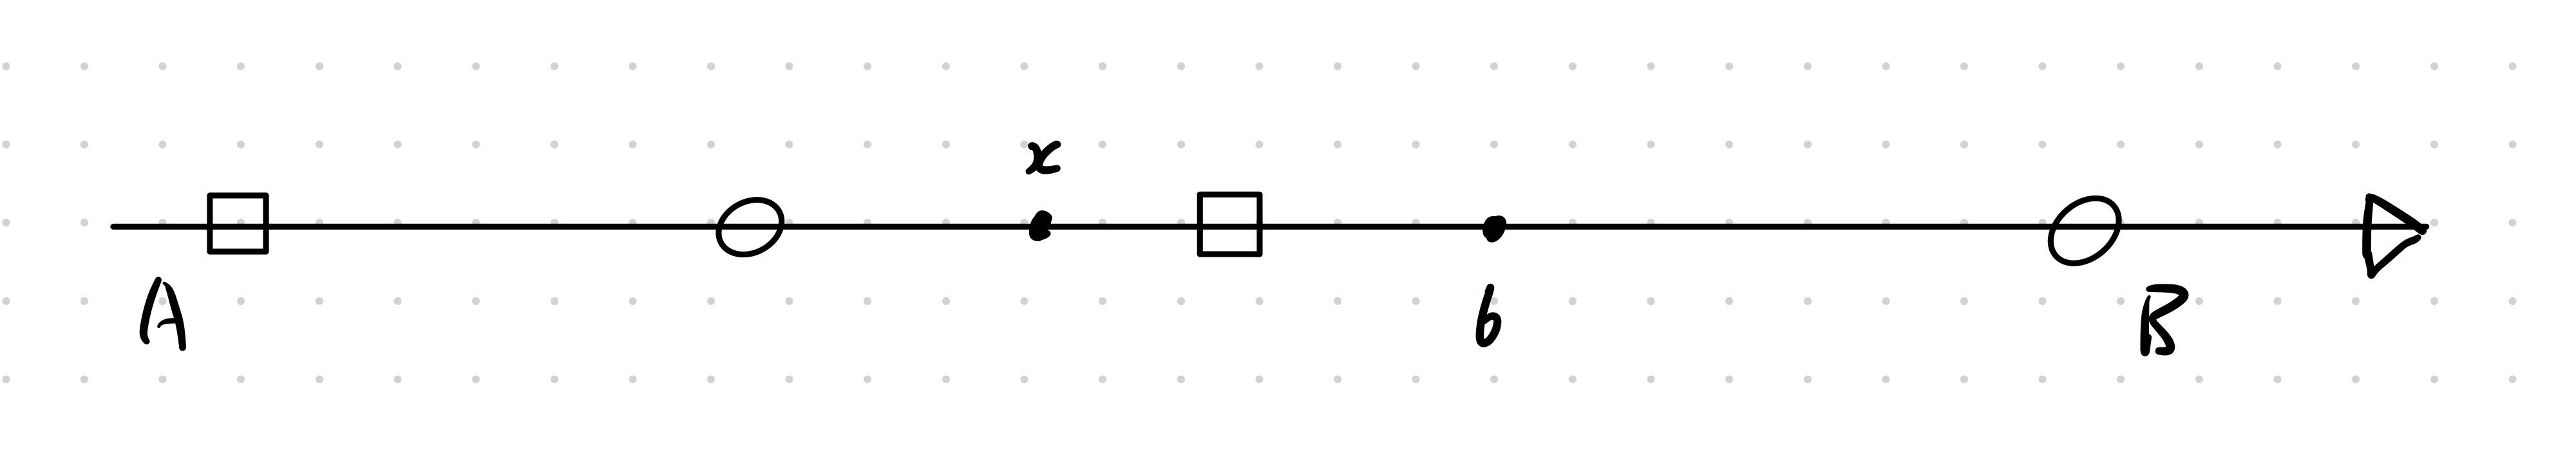
\includegraphics[width=\textwidth]{b_over_a.jpg}
    \begin{align*}
        &\text{If } x \in A \cap B \text{, then}\\
        &\exists b \in B \text{ s.t. } a < b, \forall a \in A && \implies b \notin A\\
        & && \implies x < b \text{ (since } x \in A \text{) and } a < b
    \end{align*}

    Simultaneously considering condition (c),

    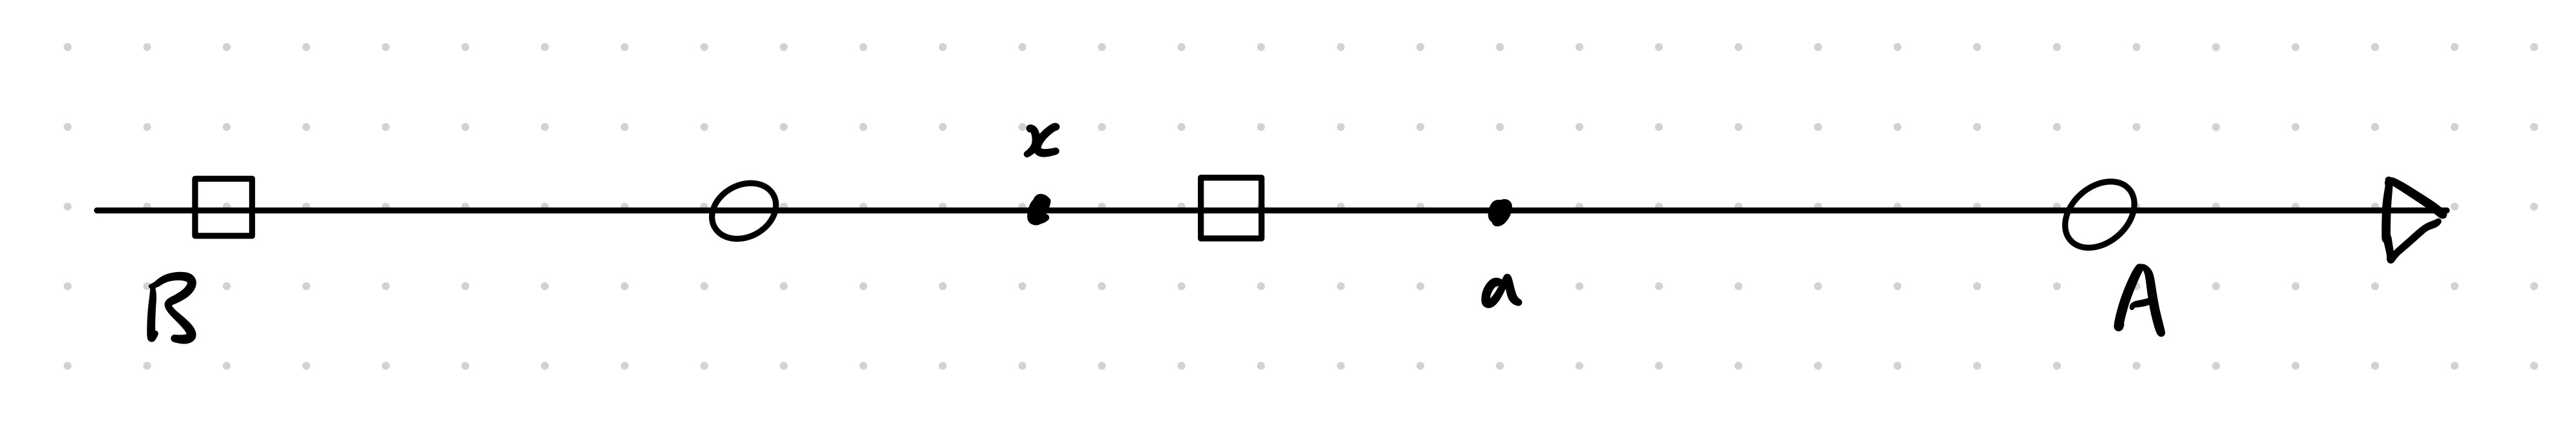
\includegraphics[width=\textwidth]{a_over_b.jpg}
    \begin{align*}
        &\text{If } x \in A \cap B \text{, then}\\
        &\exists a \in A \text{ s.t. } b < a, \forall b \in B && \implies a \notin B\\
        & && \implies x < a \text{ (since } x \in B \text{) and } b < a
    \end{align*}

    %\newpage
    This leaves us with four states which must be simultaneously true:

    \[
        \forall x \in A \cap B, \exists a \in A, b \in B \text{ such that: }
    \]
    \begin{enumerate}
        \item $x < b$.
        \item $x < a$.
        \item $a < b$.
        \item $b < a$.
    \end{enumerate}
    This implies $a < b < a \Rightarrow a < a$ which is not possible unless $A = \phi$
    and $B = \phi$ via vacuous truth, which contradicts condition (a).
\end{proof}
\end{document}